% ----------------------------------------------------------
\chapter{Conceituação e Revisão Bibliográfica}\label{cap:conceitos}

Ao longo deste capítulo serão introduzidos conceitos necessários para a compreensão do algoritmo proposto como objetivo, com uma pesquisa calcada tanto em materiais e documentos históricos quanto produções acadêmicas recentes de maior relevância.

\section{Conceitos Gerais}
% ----------------------------------------------------------
Nessa seção estão descritos os conceitos que a proposta desse trabalho utiliza como alicerce para a construção do objetivo definido.

\subsection{Estegranografia}

\subsubsection{Definição e Histórico}

Etimologicamente a palavra esteganografia deriva do grego, \textit{steganographia}, que significa de forma literal "escrita escondida". Historicamente a palavra já foi utilizada para definir um conjunto bem abrangente de técnicas ao decorrer dos sećulos, iniciando-se com ocultação de símbolos em placas de hieróglifos egípicios, passando por técnicas de alteração química em tintas que só seriam exibidas em determinadas circustâncias durante a Segunda Guerra Mundial e chegando nos dias atuais com o uso de algoritmos computacionais para ocultação de mensagens em arquivos digitais.

Conceitualmente, a primeira definição registrada vem do polímata Johannes Trithemius na obra \textit{Steganographia}, escrita em 1499 e publicada apenas após sua morte em 1606 em três partes. No subtítulo do tratado, originalmente em latim e traduzido por Judge, o autor alemão introduz esteganografia como a arte pela qual a escrita é escondida e requer recuperação pela mente humana \cite{judge}.

A publicação em si é uma demonstração do uso da escrita escondida, pois inicialmente foi reconhecida como um tratado sobre demonologia de teor teológico, e só após um estudo mais aprofundado foram encontradas mensagens escondidas com metodologia sofisticadas nos dois primeiros livros. O terceiro livro só foi decifrado em 1998 por Thomas Ernst \cite{ernst} e Jim Reeds \cite{reeds} que trabalharam sem conhecimento da pesquisa um do outro.

Com a evolução da área e do campo científico como um todo, se fez necessário definir esteganografia de forma menos esotérica do que a usada por Trithemius. De forma objetiva, esteganografia é o uso de qualquer processo capaz de ocultar a existência de uma mensagem em um objeto externo, tornando essa mensagem opaca para qualquer observador que não tenha o conhecimento prévio da aplicação da técnica \cite{judge}. 

Segundo Katzenbeisser (1999) podemos generalizar grande parte dos métodos esteganográficos em um princípio comum: o remetente deseja compartilhar uma mensagem secreta (\textit{m}) com um receptor pré informado, para isso ele escolhe um \textbf{objeto de cobertura} (\textit{c}) que possa ser visto como uma mensagem pública. Então, utilizando-se de algum método específico, o remetente insere \textit{m} dentro de \textit{c}. Pode-se ainda utilizar uma \textbf{estego-chave} (\textit{k}) para controlar o processo de inserção de \textit{m}. O resultado desse processo é chamado de \textbf{estego-objeto}, e deve ter uma estrutura que permita a extração de \textit{m} desde que \textit{k} (caso exista) seja conhecido, sem que seja necessário conhecer o \textit{c} original. Uma mesma cobertura não deve ser utilizada duas vezes, já que um atacante em posse de duas versões de \textit{c} pode utilizar as divergências entre elas para detectar a existência de uma mensagem e possivelmente recuperar \textit{m} \cite{petitcolas}. Tal esquema está ilustrado na Figura 1.

\begin{figure}[!htb]
     \centering
     \caption{Diagrama geral de um método esteganográfico.}
     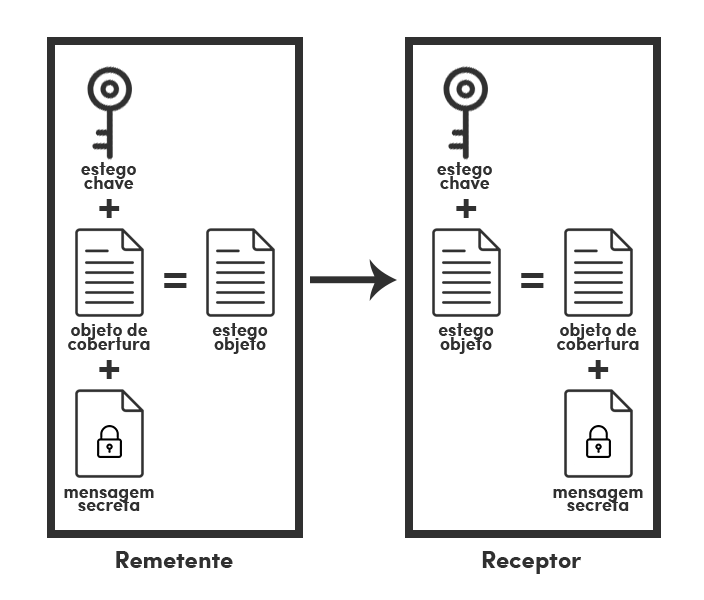
\includegraphics[width=13cm]{images/TCC1.png}
     \legend{Fonte: Imagem produzida pelo Autor}
     \label{fig_steg}
\end{figure}

\subsubsection{Tipos de Esteganografia}

Como citado anteriormente, a chave \textit{k} é opcional, sendo que sua presença e tipo podem classificar um método de esteganografia em 3 classes: esteganografia pura, esteganografia de chave privada e esteganografia de chave pública. Caso não exista uma chave, então temos uma esteganografia pura onde não há nenhuma troca de informações secretas anterior à comunicação. Apesar de possuírem implementações normalmente mais simples, métodos de esteganografia pura ferem o segundo princípio de Kerckhoffs \cite{Kerckhoffs1883}, que aconselha que a segurança de um sistema de cifragem seja baseada em uma chave e não no algoritmo de cifragem, dessa forma caso o funcionamento do sistema seja conhecido pelo atacante, ele ainda não é capaz de quebra-lo sem a chave. Por consequência disso, o recomendado é que se utilizem os métodos baseados em chaves.

 Na esteganografia de chave privada, é necessário que as duas partes compartilhem uma única chave que será utilizada durante o processo de inserção da mensagem secreta, de forma impossibilitar que qualquer atacante sem possa da chave seja capaz de decifrar a mensagem mesmo que tenha conhecimento do algoritmo. Essa classe possui conceitos que são análogos à criptografia simétrica, herdando portanto seus contratempos, sendo o principal deles a necessidade de um canal seguro para que a chave privada seja compartilhada antes do início da comunicação \cite{anderson}.

 A terceira classe de métodos é derivada da criptografia assimétrica, exigindo de um par de chaves, uma pública e uma privada. Durante o processo de inserção dos dados no objeto de cobertura, a chave pública é utilizada, enquanto para a recuperação da mensagem original é usada a chave privada. Pode-se inclusive construir um método de esteganografia de chaves públicas em cima de uma base de um sistema criptográfico de chaves públicas \cite{anderson}.

 \subsubsection{Aplicações Modernas}

 Em tempos anteriores à popularização de computadores a esteganografia possuía um leque de aplicações fortemente confinado à transmissão de mensagens secretas entre dois correspondentes. A razão disso passa primeiramente pela falta de eficiência nos métodos utilizados, e em seguida pelo fato de que as aplicações modernas que conhecemos hoje sequer eram um assunto existente na sociedade da época.
 
 O campo de marcas d´água digitais surge com a necessidade de inserir e verificar provas de autoria e propriedade de recursos digitais, e avança conforme as legislações específicas de grandes países ou blocos são sancionadas. Entretanto, nessa área os requisitos para a utilização de um algoritmo diferem dos habituais, dado que existe a necessidade de impedir que a marca seja retirada ou corrompida por transformações no arquivo. Além disso, a invisibilidade completa da mensagem nem sempre é indispensável e podemos ter marcas d'água visíveis para um observador externo. Mesmo com essas ressalvas, é notório que os últimos anos de evolução das técnicas de esteganografia foram fortemente voltados para aplicações na área de marcas d´água digitais, por seu apelo comercial latente \cite{9187785}.
 
 Apesar da natureza distinta entre as duas áreas, grande parte dos algoritmos utilizados para esteganografia podem ser transpostos para a aplicação de marcas d´água, visto que possuem a robustez necessária para impedir a mensagem de ser violada e que a ocultação da mesma não é um impeditivo \cite{9187785}. E, de fato, possuímos exemplos de usos extensivos como os micropontos invisíveis a olho nu adicionados por impressoras comerciais em suas impressões \cite{10.1145/2656434.2656437} e as câmeras digitais com capacidade de adicionar uma marca invisível em cada foto que tiram \cite{blythe}.

 \subsubsection{Problema dos Prisioneiros}

 Formulado por Simmons, o problema dos prisioneiros é um modelo utilizado para para descrever comunicação subliminar a partir de um canal monitorado. No problema os dois prisioneiros Armando e Bruna estão confinados em celas diferentes e Chico, o carcereiro, inspeciona toda a comunicação entre eles, descartando qualquer tipo de mensagem criptografada ou de conteúdo suspeito, forçando os dois a traçarem seu plano de fuga utilizando apenas comunicação invisível \cite{Simmons1984}. Podemos assumir que em um momento anterior à prisão, os dois prisioneiros combinaram uma chave a ser utilizada para algum tipo de comunicação e que o carcereiro atua de forma passiva apenas validando as mensagens sem alterá-las. Além disso, assumimos que o canal de comunicação é conhecido por Chico, para obedecer ao segundo princípio de Kerckhoffs.

 Dessa forma podemos utilizar o diagrama exposto na Figura \ref{fig_steg} para descrever uma troca de mensagens dentro do problema dos prisioneiros. Em uma cela, Armando escolhe uma mensagem inocente que será utilizada como objeto de cobertura e insere a mensagem secreta processada a partir da estego chave, gerando um estego objeto que é passado pelo canal de comunicação monitorado por Chico, e em outra cela, Bruna recebe o estego objeto e reconstrói a mensagem secreta a partir da chave combinada. Caso essa comunicação seja feita sem que o carcereiro consiga detectar a existência de uma mensagem no estego objeto podemos dizer que ela foi bem sucedida e invisível. Ao longo desse trabalho iremos utilizar esse problema de forma a buscar uma solução satisfatória para ele. 

\subsection{Arquivos Executáveis}

A esmagadora maioria das pessoas programadoras atualmente escreve código em linguagens de alto nível que são muito próximas de línguas humanas, enquanto computadores modernos interpretam sequências de instruções representadas em base binária. Isso só é possível graças a compiladores, softwares que transformam construções feitas em linguagens de alto nível para o que chamamos de linguagem de máquina \cite{patterson}.

O processo de compilação usualmente toma como parâmetros de inicialização um código fonte escrito em uma linguagem de alto nível e produz um arquivo, comumente chamado de arquivo executável. Esse arquivo é capaz de ser carregado para o processador e executar as instruções dadas pelo programa. Esses arquivos podem possuir estruturas e formatos diferentes, dependendo do sistema operacional e do processador alvos que foram usados. Atualmente os dois formatos mais utilizados são o ELF e PE, utilizados respectivamente pelos sistemas operacionais Linux \cite{linuxbase_4} e Windows \cite{microsoft_pe}. Apesar de possuirem diferenças, ambos os formatos citados compartilham características. Além do código já devidamente representado em linguagem de máquina, os arquivos carregam um cabeçalho com metadados referentes ao programa.

\subsubsection{ELF (\textit{Executable and Linkable Format})}

O formato ELF foi desenvolvido inicialmente pela Unix System Laboratories em 1988, ganhando notoriedade e implementações em outros sistemas, até que em 1999 foi adotado como padrão pelo sistema Unix e seus derivados. Por ser facilmente generalizado para diversos tipos de sistemas e possuir suporte para a maioria das funcionalidades utilizadas pela indústria atualmente, continua até hoje figurando entre os formatos mais relevantes para arquivos executáveis.

Estruturalmente, um arquivo ELF é dividido em duas estruturas principais: segmentos e seções. Os segmentos contém informações úteis para o programa durante seu tempo de execução, como o local e valores de constantes definidas em código e as próprias instruções do programa. As seções possuem dados utilizados em tempo de ligação ou para \textit{debugging} como símbolos gerados no processo de compilação e endereços de realocação de memória \cite{elf}.

Para organizar essas informações, é utilizado um esquema de cabeçalhos contendo metadados e posições dos segmentos e seções. Logo no início do arquivo está o \textit{ELF Header} detalhando informações como arquitetura alvo, tipo de arquivo e posições para os próximos cabeçalhos. Em seguida começam os \textit{Program Headers} que definem como estão dispostos os segmentos no arquivo, os próprios segmentos e seções com seus conteúdos e por fim os \textit{Section Headers} contendo as informações das seções. A estrutura típica de um executável contendo código e dados pode ser vista na figura a seguir, notando que é comum essa sobreposição entre secções e segmentos na memória \cite{elf}.

\begin{figure}[!htb]
     \centering
     \caption{Estrutura de um arquivo ELF contendo dados e código.}
     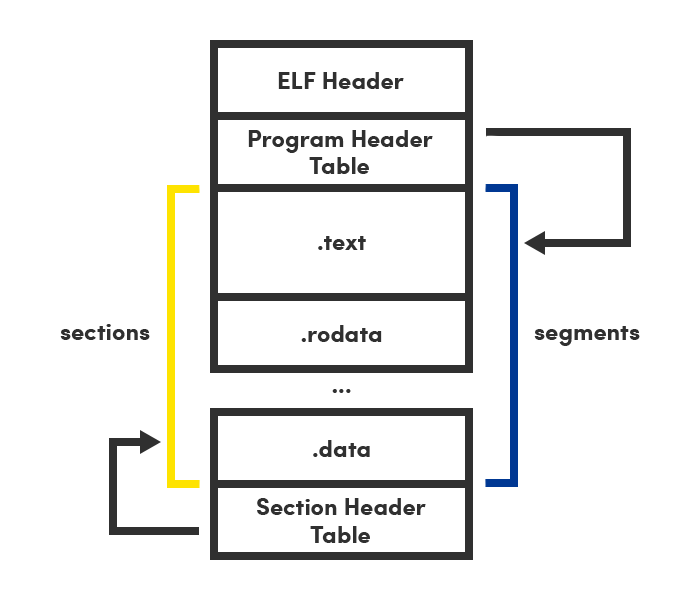
\includegraphics[width=13cm]{images/TCC2.png}
     \legend{Autor: Imagem produzida pelo Autor}
     \label{}
\end{figure}

\subsection{Arquitetura RISC-V}

Assim como nem todos os humanos compreendem a mesma língua, nem todas as máquinas sabem interpretar a mesma linguagem. Existem diversas formas de representar a linguagem de máquina desenvolvidas ao passar das décadas por diferentes fabricantes de computadores, cada máquina possuindo seu próprio conjunto de instruções que é capaz de executar. Esse conjunto é comumente denominado \textit{Instruction Set Architecture} (ISA) e todas as máquinas que compreendem um mesmo conjunto são ditas da mesma arquitetura.

Atualmente duas grandes filosofias de construção de arquiteturas disputam espaço no mercado, \textit{Complex Instruction Set Computer} (CISC) e \textit{Reduced Instruction Set Computer} (RISC), tendo como mote principal a complexidade do seu conjunto de instruções. Enquanto máquinas CISC possuem um conjunto de instruções maior e essas instruções também contém um grau de complexidade mais elevado, as máquinas RISC possuem poucas operações e buscam realizar as operações de forma fragmentada em uma quantidade maior de passos simples \cite{patterson_risc_i}.

Em consequência dos princípios básicos de cada tipo de máquina, é possível inferir características que serão comuns a todas as arquiteturas de cada classe. Máquinas CISC costumam gerar códigos menores, pois aglutinam diversas operações em uma só instrução, enquanto nas implementações RISC temos o oposto. Entretanto, apesar da quantidade total de instruções geradas para um mesmo código na máquina RISC ser maior, cada instrução possui uma execução mais rápida devido a sua simplicidade, retomando de volta a performance perdida por executar um número maior de instruções \cite{patterson_risc_i}.

Nos dias atuais a melhor representação de uma arquitetura CISC é a x86, desenvolvida inicialmente pela Intel em 1978 como uma extensão da arquitetura 8080. Apesar de ser coloquialmente referida como uma arquitetura, é na verdade um conjunto que abarca diversas ISAs desenvolvidas ao longo das décadas. Para máquinas RISC podem ser citadas as arquiteturas \textit{Advanced RISC Machine} (ARM) e RISC-V, sendo que a última possui esse nome por ser a quinta geração de arquiteturas RISC a ser desenvolvida pela Universidade da Califórnia.

A arquitetura RISC-V é uma ISA desenvolvida de forma aberta e sem cobrança de \textit{royalties}, originalmente pelo departamento de engenharia elétrica e ciências da computação da Universidade da Califórnia, campus Berkeley. Entretanto, desde o início em 2010 até o presente, muitos contribuidores externos, independentes ou em contribuições corporativas, participaram do projeto. Diferentemente do usual para projetos acadêmicos, o RISC-V busca não apenas ser um objeto de estudo teórico, mas também ter viabilidade para projetos reais na indústria \cite{Asanović:EECS-2014-146}.

O RISC-V possui um conjunto de apenas 47 instruções obrigatórias, complementadas por extensões padronizadas de propósitos gerais que adicionam funcionalidades como multiplicação, operações atômicas e aritmética de ponto flutuante. Todas as operações são realizadas exclusivamente em registradores, utilizando o conceito de \textit{load/store machine}, para operar sobre um valor em memória primeiro é necessário uma instrução para carregá-lo em um registrador, em seguida é realizada a operação em uma segunda instrução, e por fim uma última instrução retorna o valor para a memória \cite{Waterman:EECS-2014-54}.

Seguindo princípios da filosofia RISC e utilizando erros de experiências passadas para aprimorar o novo projeto, atualmente o RISC-V é considerado por grande parte da comunidade como o futuro do \textit{hardware open source}, possibilitando que universidades, indivíduos e empresas possam criar implementações completamente livres em cima de uma base sólida.

\section{Trabalhos Relacionados}

Apesar de não ser um assunto extensamente explorado, a esteganografia utilizando código executável já foi proposta e estudada por outros autores ao longo dos últimas décadas.
O projeto Hydan utiliza instruções semânticamente equivalentes como decisores binários para inserir dados dentro de um código executável para a arquitetura x86. Entretanto, a razão de codificação de em média 1 bit de mensagem para cada 100 bits do objeto de cobertura encontrada é insatisfatória para alguns casos de uso \cite{Hydan}. No mesmo ano, Anckaert \textit{et al} (2004) expandem o conceito inicial do Hydan, realizando um estudo sobre a redundância em programas da arquitetura x86 e formulando critérios de substituição claros. Além disso, esse trabalho também traz um \textit{framework} para análise de detectabilidade dos estego-objetos gerados.

O \textit{whitepaper} publicado por Wright (2008) desenvolve em cima de um tópico já citado pelos autores originais do Hydan: a fragilidade do trabalho em relação a detectabilidade. O método aplicado pelos pesquisadores não leva em consideração a distribuição estatística das instruções em cada plataforma, permitindo que uma análise seja feita buscando anomalias, comparando instruções contidas no programa alvo com a distribuição normalmente encontrada em programas compilados para a mesma plataforma \cite{Wright2020DetectingHS}.

Outra abordagem foi tomada por Shin \textit{et al} (2008), que desenvolve um método para inserção de dados em arquivos do formato PE, adicionando os dados na seção \textit{.text} do binário e tomando providências de realocação caso seja necessário. Apesar desse método possuir uma flexibilidade maior e capacidade de codificação virtualmente infinita, ele altera o tamanho do arquivo em disco, portanto pode ser detectado por um observador externo em posse do objeto de cobertura, invalidando essa técnica para aplicações em que o arquivo original seja de alguma forma público. De forma complementar, um trabalho posterior propõe um método similar cobrindo as mesmas plataformas e adicionando uma camada de criptografia \cite{zaidan}.

Além de métodos diferentes para a inserção dos dados no objeto de cobertura, a natureza dos próprios dados é espaço de pesquisas. Lu, Xiong e Gao (2014) elaboraram a ideia de utilizar esteganografia não só para esconder uma mensagem dentro de um código fonte, mas sim para esconder parte do código fonte dentro de si mesmo. Os autores utilizam \textit{Return Oriented Programming} (ROP) em combinação com esteganografia para que certos conjuntos de instrução sejam invisíveis à analisadores estáticos de código mas ainda sejam executadas em tempo de execução. Como prova de conceito é apresentada a ferramenta RopSteg que utiliza uma versão modificada do algoritmo de \textit{Galileo} para gerar segmentos de código contendo estruturas de retorno que não estavam no binário original. Entretanto, apesar de conseguirem êxito para fazer as alterações no arquivo, devido à ROP ser frequentemente associada com malwares, os autores alertam que existe a possibilidade do arquivo gerado ser marcado como malicioso por sistemas de detecção \cite{ropsteg}.

Por fim, existem ainda implementações não acadêmicas porém relevantes, utilizando propostas levantadas pelos autores anteriores e que de certa formam fornecem alguma validação da viabilidade material desses métodos. A ferramenta \textit{steg86} apropria-se da ideia inicial dos autores do Hydan para desenvolver uma interface de linha de comando simples para ocultação de dados em binários compilados para as plataformas x86 e AMD64, oferecendo suporte tanto para ELF quanto para PE. Além de operações básicas de injeção e extração de mensagens, o utilitário também oferece um comando para fazer uma análise de um binário e determinar quantos bits podem ser inseridos nele \cite{steg86}.